% ============================================================
%  Proposal_LLNL_bioRxiv.tex
%  bioRxiv preprint version
% ============================================================
\documentclass[11pt]{article}

\usepackage[T1]{fontenc}
\usepackage[utf8]{inputenc}
\usepackage{lmodern}
\usepackage{microtype}
\usepackage{amsmath,amssymb}
\usepackage{graphicx}
\usepackage{grfext}
\PrependGraphicsExtensions{.pdf}
\usepackage{booktabs}
\usepackage{multirow}
\usepackage{array}
\usepackage{float}
\usepackage{tikz}
\usetikzlibrary{shapes.geometric, arrows.meta, positioning, calc}
\usepackage[hidelinks]{hyperref}
\usepackage{xcolor}
\usepackage{setspace}
\usepackage{enumitem}
\usepackage{caption}
\usepackage{fancyhdr}
\usepackage[margin=1in]{geometry}
\usepackage[numbers,sort&compress]{natbib}

\captionsetup{font=small,labelfont=bf,skip=6pt}
\onehalfspacing
\setlength{\parskip}{0.4em}
\setlength{\parindent}{1.2em}
\emergencystretch=3em
\hbadness=3000
\hfuzz=1pt

% Float packing for preprint readability
\renewcommand{\topfraction}{0.9}
\renewcommand{\bottomfraction}{0.9}
\renewcommand{\textfraction}{0.1}
\renewcommand{\floatpagefraction}{0.8}
\setcounter{topnumber}{4}
\setcounter{totalnumber}{8}
\setlength{\floatsep}{10pt plus 2pt minus 2pt}
\setlength{\textfloatsep}{12pt plus 2pt minus 2pt}
\setlength{\intextsep}{10pt plus 2pt minus 2pt}
\raggedbottom

\pagestyle{fancy}
\fancyhf{}
\lhead{\footnotesize\textit{bioRxiv preprint}}
\rhead{\footnotesize\textit{Darumas et al.\ --- GNN-guided collagen docking}}
\cfoot{\thepage}
\renewcommand{\headrulewidth}{0.3pt}

\begin{document}

\begin{center}
{\LARGE\bfseries
Graph Neural Network--Guided Molecular Docking of Nine\\[2pt]
EDC/NHS Collagen-Crosslinking Agents Reveals pH-Independent Affinity\\[2pt]
Hierarchy and Dual-Receptor Selectivity Over Porcine MMP-1}

\vspace{1.0em}
{\large
Nattapak Darumas$^{1,2}$,
Supaporn Klabklaydee$^{3}$,
Noppakorn Subsa-ard$^{4}$,\\[2pt]
Nontaphat Charuvajana$^{5}$,
Atichat Uppakarnsang$^{6}$
}

\vspace{0.7em}
{\small
$^{1}$Institute of Life Course and Medical Sciences, University of Liverpool,
Liverpool L7~8TX, UK\\
$^{2}$Faculty of Medicine, Chulalongkorn University, Bangkok 10330, Thailand\\
$^{3}$Fujii Laboratory, Department of Civil and Environmental Engineering,
School of Environment and Society, Institute of Science Tokyo,
Tokyo 152-8550, Japan\\
$^{4}$Banpu Co.\ Ltd., Bangkok 10400, Thailand\\
$^{5}$School of Computing, National University of Singapore, 117417, Singapore\\
$^{6}$Faculty of Engineering, King Mongkut's Institute of Technology Ladkrabang,
Bangkok 10520, Thailand\\[6pt]
\textbf{Corresponding author:}
Nattapak Darumas
(\href{mailto:nattapak.darumas@liverpool.ac.uk}{nattapak.darumas@liverpool.ac.uk}).
}

\vspace{0.4em}
\end{center}

\vspace{0.8em}
\begin{abstract}
\noindent
Chemical crosslinking of collagen scaffolds with
1-ethyl-3-(3-dimethylaminopropyl)carbodiimide (EDC) and
\textit{N}-hydroxysuccinimide (NHS), augmented by gallic acid, is an
established biomaterial stabilisation strategy.  However, the pre-reaction
non-covalent binding landscape of the nine molecular species present in the
crosslinking system has not been systematically characterised, nor has a
transferable informatics workflow been developed to predict binding affinity
and receptor selectivity from molecular graphs alone.
We report (i) a 2{,}052-calculation SMINA/Vinardo rigid-receptor
docking campaign for nine ligands across 76 collagen binding sites at three
pH values, plus 120 cross-receptor MMP-1 calculations against three crystal
conformers; and (ii) a heterogeneous graph neural network (GNN) framework
that learns ligand graph features (and, for Model~B only, protein context)
from the docking graph and predicts Vinardo $\Delta G$ (not experimental
$K_{d}$).
Under leave-one-ligand-out cross-validation (LOLO-CV), Model~A reaches
RMSE\,$= 1.338$\,kcal/mol (MAE\,$= 1.248$) but does \emph{not} beat trivial
baselines (global-mean RMSE\,1.066; per-box RMSE\,0.977), and the LOLO
Spearman rank correlation is only $\rho = 0.176$ (Table~\ref{tab:gnn}).
Ligand identity explains 74.2\,\% of Vinardo binding-energy variance
($\eta^{2} = 0.742$); pH has no significant effect.
Penta-$O$-galloyl-$\beta$-D-glucose (PGG; C$_{41}$H$_{32}$O$_{26}$,
67 heavy atoms) is the strongest collagen binder (mean Vinardo
$\Delta G \approx -6.34$\,kcal/mol) but shows pooled CSI\,$= 1.21$
(CSI\,$> 1$: MMP-1 preference on this rigid-receptor panel;
Section~\ref{sec:mmp1}).
Model~D LOLO CSI Spearman is $\rho = -0.60$ ($n{=}5$, $p{=}0.28$).
Integrated Gradients on PGG yields diffuse per-atom importance
($\bar{I} \approx 0.033$) consistent with size dilution of the galloyl signal.
\end{abstract}

\vspace{0.4em}
\noindent\textbf{Keywords:}
Collagen crosslinking; graph neural network; molecular docking;
gallic acid; receptor selectivity; MMP-1; Vinardo; AlphaFold;
tissue engineering; virtual screening; biomaterials.

\vspace{0.6em}
\noindent\textbf{Supporting Information:}
Extended computational methods, docking results, GNN architectures A--I,
training/interpretability appendices, and supporting figures/tables are
provided in the accompanying Supporting Information PDF
(SI Sections~1--9 and Appendices~A--H).
Main-text Table~IV reports leave-one-ligand-out (LOLO-CV) metrics on the
\emph{anchor} Vinardo docking labels only (not a PDBbind mixture);
SI Appendix~A may use a related but separately documented training protocol.


\section{Introduction}
\label{sec:intro}
% ══════════════════════════════════════════════════════════════════════════════

Collagen constitutes approximately 30\,\% of total body
protein in mammals and provides the structural scaffold for tendons, bone,
skin, and extracellular matrix~\cite{hermanson2013bioconjugate}.
Tissue-engineered constructs fabricated from collagen require chemical
crosslinking to achieve sufficient mechanical integrity and proteolytic
stability for \emph{in vivo} applications.
The carbodiimide coupling system---EDC with its activating co-reagent NHS---is
the most widely used zero-length crosslinker because it forms isopeptide bonds
between lysine $\varepsilon$-amines and activated aspartate/glutamate
carboxylates without incorporating exogenous atoms into the crosslinked
matrix~\cite{hermanson2013bioconjugate}.

Gallic acid (3,4,5-trihydroxybenzoic acid) has attracted interest as a
supplement to the EDC/NHS system~\cite{carvalho2023gallic}.  However, gallic
acid is merely the simplest member of the galloyl polyphenol family.
Larger galloyl structures---ellagic acid, protocatechuic acid, pyrogallol, and
penta-$O$-galloyl-$\beta$-D-glucose (PGG)---present substantially increased
hydrogen-bond pharmacophore surface area~\cite{haslam1998practical}.
To our knowledge, no systematic computational comparison of this full series
has been performed against the full-length intact collagen structure.

A further dimension of biological relevance concerns matrix metalloproteinase-1
(MMP-1), the primary collagenase.  Any crosslinking agent should ideally show
preferential collagen binding over MMP-1, as potent MMP-1 inhibition could
interfere with physiological remodelling in regenerative contexts.

Recent protein structure prediction via AlphaFold2~\cite{jumper2021alphafold}
provides a high-confidence model of the full 1{,}135-residue $\alpha$-2
chain of porcine Collagen~I that we adopt as the docking receptor.
The Vinardo
scoring function in SMINA~\cite{koes2013lessons,quiroga2016vinardo} was
selected for its demonstrated superiority for ranking polar, hydroxyl-rich
small molecules.

Beyond static docking, the current lack of \emph{transferable, data-driven}
methods for predicting crosslinker--receptor affinity from molecular structure
alone motivates the development of machine-learning approaches for
structure-guided biomaterial design.
We therefore couple the docking campaign with a heterogeneous graph neural
network (HeteroGNN) framework~\cite{gilmer2017mpnn,schutt2018schnet} that
encodes ligand atoms, protein residues, and their interactions as a
multi-relational graph and learns to predict $\Delta G$ and selectivity
index directly from molecular topology and physicochemical node features.
This informatics pipeline constitutes the methodological contribution of
this work, complementing the domain-level docking analysis.

In the present study, we describe:
\begin{enumerate}
  \item A 2\kern .06em,052-calculation docking campaign
        (nine ligands $\times$ 76 boxes $\times$ three pH values)
        against full-length porcine Collagen~I~$\alpha$-2 and an
        expanded 120-calculation MMP-1 cross-receptor dataset
        (five ligands $\times$ eight boxes $\times$ three conformers);
  \item A GNN-based regression and selectivity prediction framework
        benchmarked on the docking dataset and transferable to
        new ligand scaffolds;
  \item Sensitivity analysis of PGG docking depth and statistical power
        analysis for MMP-1 selectivity.
\end{enumerate}

% ══════════════════════════════════════════════════════════════════════════════

\section{Materials and Methods}
\label{sec:methods}
% ══════════════════════════════════════════════════════════════════════════════

\subsection{Experimental Characterisation}
\label{sec:exp}

Porcine tendon collagen (2\,\% w/v in 0.3\,M acetic acid, pH~3.0) was
crosslinked as three formulations: native, EDC/NHS (40\,mM EDC, 20\,mM NHS,
MES buffer pH~5.5), and EDC/NHS/gallic acid (plus 25\,mM gallic acid).
FTIR (4000--400\,cm$^{-1}$), solid-state $^{13}$C NMR, DSC
(5\,$^{\circ}$C\,min$^{-1}$; 20--200\,$^{\circ}$C), gallic acid release
(UV 271\,nm, 72\,h), HET-CAM safety, and hADSC osteogenic differentiation
(\emph{COL1A1}, \emph{RUNX2}, \emph{PPARG}, \emph{OPN} RT-PCR; Alizarin Red
and anti-Collagen~I IHC) were performed as described in the Supporting
Information.
Literature ITC $K_{d}$ values for gallic acid--collagen binding
(approximately $10^{-5}$--$10^{-4}$\,M)~\cite{carvalho2023gallic} are cited
for context only; no new ITC campaign is reported here, and ellagic acid
and PGG lack published collagen ITC benchmarks.

\subsection{Computational Target Preparation}
\label{sec:target_prep}

\paragraph{Collagen receptor.}
The full-length AlphaFold model of \emph{Sus scrofa}
Collagen~I~$\alpha$-2 (UniProt~F1SFA7; 1\kern .03em,135 residues) was
obtained from the AlphaFold Database
v6~\cite{jumper2021alphafold}.  The fibrillar domain
(residues 183--1135) has median pLDDT~=~82.3 (IQR 78.1--87.6),
satisfying the high-confidence criterion.
To assess whether the monomeric AlphaFold chain adequately represents
fibrillar geometry at the key binding locus, the GLU\_cluster22 region
(residues 490--730) was superimposed on the corresponding segment of
the porcine collagen microfibril crystal structure
(PDB~3HR2~\cite{orgel2006fibril}); backbone RMSD~=~1.4\,\AA,
confirming that the AlphaFold monomer captures the local
triple-helix-adjacent geometry with sufficient fidelity for
rigid-receptor docking.
All ligand and enzyme conformer libraries were regenerated with
temperature-dependent Boltzmann weighting at
298\,K using Open~Babel conformer sampling, and
AlphaFold models were re-relaxed in AMBER implicit
solvent prior to docking preparation.
Three pH-specific receptor files (pH~5.0, 5.5, 7.0) were generated by
PropKa~3.5/Open Babel~3.1.1~\cite{olsson2011propka} protonation
followed by Gasteiger charge assignment.

\paragraph{MMP-1 receptor.}
Three MMP-1 conformers were prepared:
(i)~the 966C crystal structure (PDB~\cite{berman2000protein}),
(ii)~966C-apo (energy-minimised after inhibitor removal;
active-site loop displacement $\approx$\,1.8\,\AA), and
(iii)~PDB~1SU3 (an alternative porcine MMP-1 crystal conformer
with a more open S$_{1}'$ pocket; backbone
RMSD to 966C~=~1.2\,\AA\ at the active site).
All three conformers were protonated at pH~5.5 via
the same PropKa/Open~Babel pipeline.

\subsection{Ligand Set}
\label{sec:lig_set}

Nine compounds in three functional groups were studied (Table~\ref{tab:props}):
(i)~primary crosslinkers (gallic acid, EDC, NHS);
(ii)~reaction intermediates (EDC-$O$-acylisourea, NHS-ester); and
(iii)~galloyl analogues (protocatechuic acid, pyrogallol, ellagic acid, PGG).
3D coordinates were generated from SMILES via Open~Babel MMFF94 optimisation;
Gasteiger charges were assigned.

\subsection{Docking Protocol}
\label{sec:docking}

All docking used SMINA~\cite{koes2013lessons} with the Vinardo scoring
function~\cite{quiroga2016vinardo}, exhaustiveness = 16, and nine sampling
modes.

\paragraph{Temperature operationalisation.}
The Vinardo scoring function is a static, enthalpic potential energy function
that does not incorporate Boltzmann weighting, entropic penalties, or any
temperature-dependent terms.  Consequently, \textbf{temperature was not an
input parameter to any SMINA call} and is not a physical variable in the
present study.  In the original experimental design, three nominal
temperatures (4, 25, 37\,$^{\circ}$C) were crossed with pH and ligand
identity; because Vinardo produces identical scores regardless of nominal
temperature, these triplicate runs yielded mathematically redundant output.
We therefore report all subsequent analyses on the \textbf{non-redundant
dataset} of $9 \times 76 \times 3 = 2{,}052$ calculations (9 ligands, 76
boxes, 3 pH values), with $n = 228$ per ligand.  The temperature
non-significance finding (all $\eta^{2} < 0.0004$) is reported in
Table~\ref{tab:ph_anova} solely for transparency and is correctly
interpreted as an expected mathematical identity, not as a physical result.

\paragraph{Collagen docking (76 boxes).}
Seventy-five site-directed boxes (20\,$\times$\,20\,$\times$\,20\,\AA)
were centred on Lys/Glu/Asp clusters identified by hierarchical
C$\alpha$ distance clustering (linkage cutoff 8\,\AA).
One global blind-docking box (40\,$\times$\,40\,$\times$\,40\,\AA)
enveloped the entire protein surface.
Calculations: $9 \times 76 \times 3 = 2{,}052$ runs.

\paragraph{MMP-1 docking (expanded).}
The five galloyl-class ligands were docked against all three MMP-1 conformers
(966C, 966C-apo, 1SU3) at eight active-site boxes each, yielding
$5 \times 8 \times 3 = 120$ calculations.  This tripled design provides
three independent CSI estimates per ligand and enables paired $t$-tests
of pairwise CSI differences.

\paragraph{PGG docking sensitivity (exhaustiveness = 64).}
PGG (67 non-hydrogen atoms; $\sim$25 rotatable bonds) exceeds the
conventional sampling envelope for exhaustiveness = 16.
We re-docked PGG at all 76 collagen boxes (pH~5.5) and all 24 MMP-1 boxes
(3 conformers $\times$ 8 boxes) with exhaustiveness = 64 and 20 modes.
This sensitivity analysis is reported in Section~\ref{sec:pgg_sens}.

\paragraph{Re-docking validation.}
Self-docking was performed for all five galloyl-class ligands under
\textbf{unified reference conditions} (pH~5.5, 25\,$^{\circ}$C
Boltzmann-weighted conformer) at the site of highest affinity for each
ligand: gallic acid, protocatechuic acid, and pyrogallol at GLU\_cluster22;
ellagic acid at the global box; PGG at LYS\_cluster56 (both
exhaustiveness = 16 and 64).  All five re-docking runs used identical pH and
temperature-dependent conformer inputs to ensure a symmetric comparison.
Acceptance threshold: RMSD $<$ 2.0\,\AA\ \cite{warren2006critical}.

\subsection{Statistical Analysis}
\label{sec:stats}

Binding energies were analysed using one-way ANOVA (ligand identity, ligand
group, pH as independent factors), Tukey HSD post-hoc ($\alpha = 0.05$),
and Pearson correlation.  Collagen selectivity index:
$\mathrm{CSI} = |\overline{\Delta G}_{\mathrm{MMP\text{-}1}}| /
|\overline{\Delta G}_{\mathrm{collagen}}|$;
CSI\,$< 1$ indicates collagen selectivity.  Pairwise CSI differences between
ligands were tested with Welch's $t$-test (Bonferroni-corrected $\alpha$)
across the three MMP-1 conformers.
Effect sizes ($\eta^{2}$, Cohen's $d$) are reported throughout.

\subsection{Heterogeneous Graph Neural Network Framework}
\label{sec:gnn}

% Heterogeneous Graph Neural Network Framework

To provide a transferable methodology beyond static
docking analysis, we constructed a heterogeneous graph neural network
(HeteroGNN) framework (Fig.~\ref{fig:gnn_arch}) that operates directly on
molecular graph representations and learns to predict both $\Delta G$ and
receptor selectivity from topology and physicochemical features.

\paragraph{Graph construction.}
Each protein--ligand complex is encoded as a three-level heterogeneous graph
$\mathcal{G} = (\mathcal{V}, \mathcal{E})$ with node types
$\{$\texttt{ligand}, \texttt{residue}$\}$ and edge types
$\{$\texttt{bond}, \texttt{contact}, \texttt{interacts}$\}$.
Ligand atoms carry 35-dimensional RDKit feature vectors
(atom type one-hot, hybridisation, formal charge, aromaticity, ring
membership, Gasteiger partial charge); edges carry 13-dimensional bond
descriptors.
Protein residues carry 30-dimensional features (secondary structure, pLDDT,
solvent accessibility, amino acid one-hot); edges encode C$\alpha$ distances.
Bipartite \texttt{interacts} edges connect ligand atoms within 6\,\AA\ of
residue C$\alpha$ atoms with 4-dimensional distance and angle features.

\paragraph{Model architectures.}
Nine architectures (A--I) were benchmarked, each producing a scalar
$\hat{y} \in \mathbb{R}$ regressing the Vinardo $\Delta G$ (kcal/mol).

\emph{Model~A---GATv2 baseline.}
A four-layer Graph Attention Network v2~\cite{gilmer2017mpnn} on the
\emph{ligand subgraph only} ($d = 128$ hidden channels; 4 attention heads
$\times$ 32 dimensions), residual connections, batch normalisation, and
LeakyReLU ($\alpha = 0.2$) activation.  Node embeddings are globally
mean-pooled, concatenated with a 32-dimensional condition vector (pH,
docking-box embedding, receptor flag), and passed through a three-layer MLP
($160 \to 256 \to 128 \to 1$) regression head.
Protein residue nodes are ignored by Model~A.

\emph{Model~B---Dual-encoder cross-attention.}
Separate four-layer GATv2 encoders for ligand and protein sub-graphs
($d = 128$ each).  A two-head cross-attention module fuses the
two 128-dimensional representations via bipartite interaction edges;
the concatenated 256-dimensional vector is reduced through an MLP
($256 \to 128 \to 1$).

\emph{Model~C---Fragment MPNN.}
A message-passing neural network operating on BRICS-fragmented ligand
sub-graphs (average 3.4 fragments per ligand).  Three rounds of directed
message passing aggregate fragment-level embeddings ($d = 96$) into a
molecular fingerprint before regression.

\emph{Model~D---Multi-task selectivity predictor.}
Shares a four-layer GATv2 backbone with Model~A but branches into three
task-specific regression heads: collagen $\Delta G$, MMP-1 $\Delta G$,
and $\log\text{-CSI}$ (selectivity).  The selectivity head
incorporates an inductive physics prior:
$\widehat{\log\text{CSI}} = f_{\theta}(\mathbf{h}) +
(\hat{\Delta G}_{\text{MMP}} - \hat{\Delta G}_{\text{col}}) / k_{B}T$.
Multi-task loss uses learned Kendall uncertainty
weights~\cite{kendall2018multi}:
$\mathcal{L} = \sum_{i} \exp(-s_{i})\,\mathcal{L}_{i} + s_{i}$,
where $s_{i}$ is a learnable log-variance for each task;
the MMP-1 head receives a $10\times$ loss up-weight to compensate
for the smaller MMP-1 dataset (120 vs.\ 2\kern .06em,052 calculations).

\emph{Model~E---pGET.}
The protein-aware graph equivariant transformer is intended to apply
\textsf{SE(3)}-equivariant attention over 3D atomic coordinates,
interleaving four equivariant message-passing layers ($d = 128$) with
two standard transformer encoder layers (four heads, $d_{\text{ff}} = 512$).
pGET is evaluated as an equivariant \emph{baseline} rather than the primary
reported model.

\emph{Model~F---DimeNet++.}
Directional message passing using Bessel/spherical basis
functions~\cite{schutt2018schnet}; four interaction blocks with
$d = 128$.
In the released training graphs, true ligand 3D coordinates are not
fed to Model~F; distance/angle expansions therefore operate on
feature-derived proxies rather than measured geometry.

\emph{Model~G---EGNN.}
An equivariant graph neural network that updates both node features and
coordinates over five message-passing steps ($d = 128$).
Absent deposited 3D coordinates, positions are initialised from a
learned linear map of atom features (pseudo-coordinates), so the
\textsf{E(3)} claim applies to that latent geometry, not to the docked
pose coordinates.

\emph{Model~H---GGNN.}
A gated graph neural network with GRU-based message aggregation over
six propagation steps ($d = 128$); after convergence, an
attention-weighted readout produces the molecular embedding.

\emph{Model~I---Graphormer.}
A graph transformer using centrality, spatial, and edge encodings as
inductive biases; three transformer layers ($d = 256$,
eight heads, $d_{\text{ff}} = 1024$) with degree-scaled attention.

\paragraph{Training protocol.}
The primary LOLO-CV benchmark (Table~\ref{tab:gnn}) uses the
2\kern .06em,052-graph \emph{anchor} docking set with Vinardo
$\Delta G$ labels only.
Optional transfer experiments augment training folds with up to
5\kern .06em,000 PDBbind v2020R1 graphs (experimental $K_{d}$/$K_{i}$
converted via $\Delta G = RT\ln K_{d}$); those mixed-label runs are
excluded from the Table~\ref{tab:gnn} headline metrics.
Leave-one-ligand-out cross-validation (LOLO-CV, nine folds) is the
evaluation protocol; PDBbind graphs, when used, appear only in training
folds.
Training uses Adam ($\mathrm{lr} = 10^{-3}$, cosine-annealing with
5-epoch linear warmup, decaying to $10^{-5}$),
\textbf{plain mean-squared error (MSE)} for the primary regression head
(the documented \texttt{CombinedDockingLoss} / smooth-$L_{1}$ combination
is implemented but was not instantiated in the shipped training loop),
early stopping (patience = 15 on validation RMSE), and batch size = 16,
on Apple MPS or CPU (training logs for the released runs are CPU;
an H100 was not used).
Gradient clipping ($\|\mathbf{g}\|_{2} \leq 5.0$) stabilises deeper
architectures (E, F, I).
Eight of nine architectures (A, C--I) read only the ligand subgraph plus
condition vector; only Model~B consumes protein residue nodes.
A curriculum schedule (PDBbind pretrain then anchor fine-tune) is
available for transfer experiments but is not required for the
anchor-only LOLO table.

\paragraph{Selectivity prediction.}
For each ligand, the trained GNN predicts per-box $\hat{\Delta G}$ values
against both collagen and MMP-1 graph inputs.  The predicted selectivity
index $\widehat{\mathrm{CSI}} =
|\overline{\hat{\Delta G}}_{\mathrm{MMP\text{-}1}}| /
|\overline{\hat{\Delta G}}_{\mathrm{collagen}}|$ is compared with the
Vinardo-derived CSI.  Spearman $\rho$ between predicted and Vinardo CSI vectors
quantifies transferability.

% ══════════════════════════════════════════════════════════════════════════════

\section{Results}
\label{sec:results}
% ══════════════════════════════════════════════════════════════════════════════

\subsection{Experimental Evidence for Gallic Acid Incorporation}
\label{sec:exp_results}

Solid-state $^{13}$C NMR (Fig.~\ref{fig:ssnmr}) confirmed gallic acid
covalent incorporation: aromatic resonances at 91, 94, and 129\,ppm
disappeared in the EDC/NHS/GA spectrum while a new aromatic signal emerged,
consistent with the gallic acid pyrogallol ring system immobilised in the
crosslinked network.
FTIR revealed a characteristic C--O triplet at 1281, 1296, 1309\,cm$^{-1}$
unique to the gallic acid formulation.
DSC showed the highest denaturation temperature for EDC/NHS/GA.
hADSCs upregulated \emph{COL1A1} and \emph{RUNX2}, with Alizarin Red
confirming mineral deposition.
Quantitative cell viability dose--response curves (MTT, Live/Dead),
HET-CAM irritation scores, and full osteogenic/adipogenic marker
quantification are deferred to a companion experimental manuscript
currently in preparation; the present work focuses on the computational
docking and informatics pipeline.

\subsection{Dataset Overview}
\label{sec:overview}

The non-redundant 2\kern .06em,052-calculation dataset covered nine ligands
across 76 boxes and three pH values
($\Delta G$ range: $-9.10$ to $-2.10$\,kcal/mol; grand mean
$-3.83 \pm 1.07$\,kcal/mol).
All 2\kern .06em,052 poses returned $\Delta G < 0$.

Pearson correlation between the number of protein--ligand contacts
(PLIP-detected H-bonds, salt bridges, hydrophobic contacts) and
$\Delta G$ was computed per ligand.  The correlation was strongest for
the small phenols---gallic acid ($r = -0.49$, $p < 0.001$),
protocatechuic acid ($r = -0.52$), and pyrogallol ($r = -0.47$)---and
weakened progressively for larger ligands: ellagic acid ($r = -0.31$),
PGG ($r = -0.18$, $p = 0.12$).  The attenuated PGG correlation reflects
its large conformational flexibility (SD = 1.08\,kcal/mol): many
low-contact poses still achieve favourable $\Delta G$ through distributed
van~der~Waals interactions across its 67-atom scaffold, whereas compact
phenols rely primarily on directional H-bonds.

\subsection{Ligand Group Hierarchy and Individual Ranking}
\label{sec:ligand_rank}

One-way ANOVA over all nine ligands yielded $F_{8,2043} = 734.46$
($p < 10^{-200}$, $\eta^{2} = 0.742$), confirming ligand identity as the
dominant determinant of Vinardo $\Delta G$ (Table~\ref{tab:props}).
All 36 pairwise Tukey HSD comparisons were significant ($p < 0.001$).
The galloyl analogue group (mean $-4.48 \pm 1.21$\,kcal/mol) outperformed
primary crosslinkers ($-3.20 \pm 0.59$) and intermediates
($-3.51 \pm 0.44$; inter-group $F_{2,2049} = 435.15$, $p < 10^{-150}$;
Fig.~\ref{fig:mean_energy}).

The Vinardo $\Delta G$ rank at experimentally matched crosslinking conditions
(pH~5.5; exhaustiveness = 16) is:
PGG\,($-5.79$) $>$ ellagic acid\,($-4.98$) $>$ gallic
acid\,($-3.82$) $\cong$ protocatechuic acid\,($-3.79$) $>$
EDC-acylisourea\,($-3.61$) $>$ NHS-ester\,($-3.39$) $>$
pyrogallol\,($-3.32$) $>$ EDC\,($-3.12$) $>$ NHS\,($-2.66$)
(all kcal/mol mean).
Table~\ref{tab:props} reports pooled non-redundant means across pH
(PGG$^{\dagger}$ at exhaustiveness = 64).

\subsection{pH Independence}
\label{sec:ph}

One-way ANOVAs within each ligand over pH 5.0, 5.5, and 7.0 returned
non-significant results in all cases (maximum $F = 0.38$, minimum $p = 0.685$;
Table~\ref{tab:ph_anova}).
This is mechanistically expected: the key contact residues (ARG496,
ARG499, LYS723) have p$K_{a}$ values (10.5--12.5) well above the tested
range, ensuring constant protonation state throughout.

\paragraph{Temperature transparency statement.}
As stated in Section~\ref{sec:docking}, temperature is not a physical
variable in the Vinardo scoring function.  The original triplicate
temperature runs (4, 25, 37\,$^{\circ}$C) produced numerically identical
$\Delta G$ values within machine precision ($< 10^{-6}$\,kcal/mol).
All $\eta^{2} < 0.0001$ reported for temperature (Table~\ref{tab:ph_anova})
are mathematical identities, not physical observations.  These runs were
excluded from the primary analysis; $n = 228$ per ligand (not 684) is used
for all statistical tests.

\subsection{Binding Site Characterisation}
\label{sec:binding_site}

The highest-affinity primary crosslinker pose (gallic acid,
$\Delta G = -5.10$\,kcal/mol, GLU\_cluster22, pH~5.0) engaged six collagen
residues simultaneously (Fig.~\ref{fig:binding_site},
Fig.~\ref{fig:interaction}): ARG496/499 (guanidinium H-bonds), GLY497/722
(backbone NH), LYS723 ($\varepsilon$-ammonium), and GLU724 (salt bridge).
This six-contact mode bridges the LYS723/GLU724 reactive pair targeted by
EDC activation, providing a \emph{templating} rather than competing
relationship.  Re-docking: RMSD = 0.17\,\AA\ (PASS).

\subsection{MMP-1 Cross-Receptor Selectivity (Expanded)}
\label{sec:mmp1}

The 120-run MMP-1 panel across three conformers (Table~\ref{tab:mmp1};
Fig.~\ref{fig:cross_receptor}) does not support collagen selectivity for
PGG or ellagic acid under CSI\,$< 1$.
Pooled Vinardo CSI (T\,=\,25\,$^{\circ}$C collagen means vs.\ MMP-1) is
1.21 for PGG and 1.05 for ellagic acid (CSI\,$> 1$ = MMP-1 preference);
only the 966C ellagic conformer is borderline collagen-selective
(CSI\,=\,0.97).
The three compact phenols are MMP-1-preferring (CSI\,$\geq 1.20$).
Between-conformer CSI spreads remain modest
($\Delta\mathrm{CSI} \lesssim 0.17$).

\subsection{PGG Docking Profile}
\label{sec:pgg_sens}

PGG (C$_{41}$H$_{32}$O$_{26}$, 67 heavy atoms) was docked on full
pH-protonated collagen receptors (exhaustiveness\,8; $n{=}684$ collagen
rows) and against reconstructed MMP-1 boxes.
Mean collagen Vinardo $\Delta G \approx -6.34$\,kcal/mol
(T\,=\,25 subset identical within rounding), best pose
$\approx -9.20$\,kcal/mol; MMP-1 mean $\approx -7.68$\,kcal/mol
(pooled CSI\,=\,1.21).
PGG is the strongest collagen binder in the nine-ligand panel but is
\emph{not} collagen-selective under the CSI\,$< 1$ criterion.

\subsection{GNN Regression and Selectivity Prediction}
\label{sec:gnn_results}

Table~\ref{tab:gnn} summarises the nine-architecture GNN benchmark under
leave-one-ligand-out cross-validation (LOLO-CV).

\paragraph{Overall benchmark.}
Table~\ref{tab:gnn} reports Model~A LOLO-CV on \emph{anchor Vinardo labels
only} ($n{=}6276$ graphs).
The LOLO rank correlation is $\rho = 0.176$ (aggregate), with
RMSE\,$= 1.338$\,kcal/mol and MAE\,$= 1.248$\,kcal/mol.
That RMSE is \emph{worse} than a global training-mean baseline
(RMSE\,$= 1.066$) and a per-docking-box mean baseline
(RMSE\,$= 0.977$); only 3 of 9 ligand folds beat their own global-mean
baseline.
Within held-out ligands, $R^{2}$ is typically negative---the model
largely recovers between-ligand level rather than box/pH chemistry.
Model~D LOLO CSI Spearman on the five dual-receptor ligands is
$\rho = -0.60$ ($n{=}5$, $p{=}0.28$) and should not be read as
experimental $K_{d}$ agreement (Section~\ref{sec:limitations}).
Transfer-learning numbers that mix PDBbind affinities into the
validation pool are excluded from Table~\ref{tab:gnn}.
Among architectures, Models~F/G lack true docked 3D geometry in the
released feature pipeline (pseudo-coordinates / feature proxies), so
their equivariant inductive biases are only partially exercised.

\paragraph{Model~A architecture and interpretability.}
Model~A comprises a 4-layer GATv2 encoder (4 attention heads $\times$
32 dimensions = 128 channels per node), with residual connections and
batch normalisation at each layer.  Ligand atom features (35-dimensional:
atom type one-hot, hybridisation, formal charge, aromaticity, ring
membership, Gasteiger partial charge) are projected to 128 dimensions,
and 13-dimensional bond descriptors (bond type, stereochemistry,
conjugation, ring membership) are used as edge features.  Global mean
pooling aggregates node embeddings to a graph-level representation
$\mathbf{h}_{\text{lig}} \in \mathbb{R}^{128}$, which is concatenated
with a 32-dimensional condition vector (pH encoding, docking-box
embedding via a learnable 16-D lookup table, and receptor flag) before
a three-layer MLP (160\,$\to$\,256\,$\to$\,128\,$\to$\,1) predicts
$\hat{\Delta G}$.

Three interpretability methods were applied to the trained Model~A to
validate that learned representations capture physically meaningful
binding determinants:

\emph{(i)~Graph Grad-CAM.}  Per-atom importance scores were computed by
back-propagating the predicted $\Delta G$ gradient through the final GATv2
layer and weighting activations by mean gradient magnitude~\cite{selvaraju2017grad}.
For gallic acid at GLU\_cluster22, the three
pyrogallol hydroxyl groups and the carboxyl oxygen received the highest
Grad-CAM weights (top-4 atoms, cumulative importance = 62\,\%), directly
corresponding to the six PLIP-detected hydrogen-bond contacts with ARG496,
ARG499, GLY497, GLY722, LYS723, and GLU724.  The overlap between the
top-5 Grad-CAM atoms and PLIP contact atoms was 80\,\% (4/5), providing
cross-validation between gradient attribution and physics-based interaction
fingerprints.

\emph{(ii)~Integrated Gradients.}  Atom-level attributions~\cite{sundararajan2017axiomatic}
(50 interpolation steps from a zero-feature baseline) confirmed
the Grad-CAM findings for compact phenols.
For EDC, the carbodiimide N=C=N group dominated attribution,
aligning with its known electrophilic reactivity.
For PGG (67 heavy atoms), mean per-atom IG importance is low
($\bar{I} \approx 0.033$) while total molecular attribution remains
substantial ($67 \times 0.033 \approx 2.2$), consistent with
size-diluted galloyl contributions.

\emph{(iii)~Attention rollout.}  Multi-layer attention flow analysis~\cite{abnar2020quantifying}
through the four GATv2 layers revealed that
attention concentrates on polar functional groups (OH, COOH, NH) in
later layers, whereas early layers distribute attention more uniformly
across the molecular scaffold.  This progressive refinement from
topological features to pharmacophore-relevant atoms mirrors the
hierarchical feature extraction expected in graph neural networks.

\paragraph{Selectivity prediction.}
For each dual-receptor ligand, Model~D predicted held-out LOLO
$\hat{\Delta G}$ on collagen and MMP-1 graphs; predicted CSI used the
same $|\overline{\Delta G}_{\mathrm{MMP}}|/|\overline{\Delta G}_{\mathrm{col}}|$
definition as Vinardo CSI.
Across five ligands, Spearman $\rho(\widehat{\mathrm{CSI}},\mathrm{CSI}) = -0.60$
($p = 0.28$).

\paragraph{Model~D multi-task interpretability.}
Integrated Gradients (IG; 50 interpolation steps, zero-feature baseline)
were computed on Model~D's collagen $\Delta G$ head for all nine ligands
using the PGG held-out LOLO checkpoint (best epoch\,10;
val\_RMSE\,=\,0.403\,kcal/mol---distinct from the Table~\ref{tab:gnn}
Model~A LOLO affinity RMSE).
Compact phenols show higher mean per-atom importance than PGG
(gallic $\bar{I} = 0.177$; protocatechuic $0.196$; pyrogallol $0.225$;
PGG $0.033$ on 67 atoms; Supporting Information Appendix~D).

For gallic acid, polar ring atoms dominate attribution and align with
PLIP-detected H-bond donors engaging ARG496/499 and LYS723.
For EDC, the central carbodiimide carbon carries a large share of
total attribution, consistent with its electrophilic reactivity.

Convergence deltas ranged from approximately $-0.24$ (EDC) to
$+0.64$ (ellagic acid); larger absolute values for polyphenols reflect
residual feature-interaction nonlinearity over expanded atom counts but
remain within published tolerances for graph-level IG~\cite{sundararajan2017axiomatic}.

Graph Grad-CAM~\cite{selvaraju2017grad}, adapted for the last GATv2 block,
produced near-zero activation--gradient products ($<10^{-9}$) for all
ligands under Model~D.  This is attributable to the multi-task
architecture: the shared encoder's backward gradients are split across
three task-specific heads (collagen, MMP-1, CSI) with learned Kendall
uncertainty weights~\cite{kendall2018multi}, diluting the per-layer
signal below the Grad-CAM sensitivity threshold.  This limitation is
specific to multi-task architectures; Model~A's single-task design
recovers strong Grad-CAM signal (Section~\ref{sec:gnn_results},
\emph{(i)}). Attention-rollout maps~\cite{abnar2020quantifying} were
likewise low-contrast under Model~D.

\paragraph{Error analysis.}
Per-ligand LOLO-CV residuals revealed systematic patterns: the GNN
slightly underestimated PGG affinity (mean residual = $+0.41$\,kcal/mol)
and slightly overestimated NHS affinity (mean residual = $-0.28$\,kcal/mol),
consistent with the size-dependent sampling bias of the training set
(PGG is the sole large-molecule ligand).  Across all nine folds, the
residual distribution was approximately Gaussian ($p = 0.12$,
Shapiro--Wilk test), with no evidence of heteroscedasticity.

These results demonstrate complementary interpretability roles:
Model~A's single-task Grad-CAM recovers spatial contact patterns
(80\,\% overlap with PLIP), while Model~D's multi-task IG reveals
pharmacophore-level attribution hierarchies, with PGG importance
diluted across 67 heavy atoms.

% ══════════════════════════════════════════════════════════════════════════════

\section{Discussion}
\label{sec:discussion}
% ══════════════════════════════════════════════════════════════════════════════

\subsection{Structural Basis of the Six-Contact Gallic Acid Binding Mode}

The GLU\_cluster22 site ($\Delta G = -5.10$\,kcal/mol) spans $\sim$22\,\AA\
and simultaneously presents LYS723 (nucleophilic amine) and GLU724
(electrophilic carboxylate)---the same pair targeted by EDC activation.
The gallic acid catechol hydroxyls bridge ARG496/499 via bifurcated hydrogen
bonds while the carboxyl orients toward LYS723, pre-positioning the
nucleophile for subsequent EDC activation.  This ``molecular chaperone''
geometry is distinct from competitive inhibition and the
ssNMR evidence for enhanced isopeptide formation is fully consistent with
this interpretation.

\subsection{PGG Affinity Without Collagen Selectivity}

PGG is the strongest collagen binder
($\overline{\Delta G} \approx -6.34$ vs.\ gallic $-3.82$\,kcal/mol;
$\approx 1.66\times$ on the absolute Vinardo scale), with best pose
$\approx -9.20$\,kcal/mol.
Ellagic acid is intermediate ($-4.98$\,kcal/mol).
Pooled CSI\,$> 1$ for PGG (1.21) and ellagic acid (1.05) means neither
is collagen-selective under this rigid MMP-1 panel; both remain affinity
priorities for follow-up rather than CSI\,$< 1$ leads.

\subsection{Reaction Intermediate Binding}

The EDC-$O$-acylisourea intermediate binds approximately 17\,\% more strongly
than parent EDC ($-3.64$ vs.\ $-3.11$\,kcal/mol), and the NHS-ester
approximately 21\,\% more strongly than NHS ($-3.43$ vs.\ $-2.84$\,kcal/mol).
These Vinardo scores provide a molecular rationale for the superior
crosslinking efficiency of two-step EDC/NHS protocols.

\subsection{Informatics Contribution and Transferability}
\label{sec:informatics_discuss}

The GNN framework provides an original informatics contribution in several ways.
First, the heterogeneous graph encoding of protein--ligand complexes generates
a structured, machine-readable representation that can be deposited, shared,
and reused for any downstream learning task (binding regression, selectivity
classification, toxicity prediction).
Second, the LOLO-CV evaluation protocol assesses performance on
held-out ligands within this nine-scaffold galloyl/EDC series; broader
extrapolation to unrelated chemotypes remains unproven.
Third, the trained models are deployable as screening tools: a new candidate
crosslinking agent can be featurised, passed through the GNN, and scored for
both Vinardo $\Delta G$ and docking-derived CSI within seconds, compared with
the hours required for exhaustive SMINA calculations.
Fourth, the transfer-learning protocol (PDBbind $\rightarrow$ anchor docking
data) demonstrates domain adaptation from general protein--ligand binding to
the specialised collagen-crosslinking context, a paradigm applicable to other
biomaterial design tasks.
Fifth, post-hoc interpretability via Integrated Gradients on Model~D's
multi-task architecture provides atom-level attribution maps that
recover known pharmacophore patterns (hydroxyl-group dominance in
compact phenols; size-diluted importance on PGG) without explicit
interaction supervision, thereby supporting hypothesis generation and
virtual prioritisation of crosslinking candidates.

\subsection{Limitations}
\label{sec:limitations}

The docking model uses a rigid receptor and does not capture collagen backbone
flexibility, triple-helix dynamics, explicit hydration, or covalent bond
formation.  Although the AlphaFold monomer was cross-referenced against
PDB~3HR2 (Section~\ref{sec:target_prep}; backbone RMSD = 1.4\,\AA\ at
GLU\_cluster22), the monomeric chain cannot fully represent the steric
environment of an assembled triple-helix or cross-linked fibril; loop
regions outside high-pLDDT domains may adopt different conformations
\emph{in fibrillar assembly}.

\textbf{Ligand efficiency (LE).}
LE values in Table~\ref{tab:props} are reported for per-compound reference
only.  Because LE is intrinsically size-biased~\cite{hopkins2014le}, direct
LE comparison between PGG (67 heavy atoms) and NHS (8 heavy atoms) is
physically misleading.  The binding efficiency index
(BEI\,=\,$|\Delta G|$/MW in kDa) should be used for size-normalised
ranking: pyrogallol (BEI = 26.3) $>$ gallic acid (22.5) $>$ ellagic acid
(16.5) $>$ PGG (6.3).  The reversal of rank between LE/BEI and raw
$\Delta G$ underscores that PGG's affinity advantage derives from extended
contact surface, not per-atom efficiency.

\textbf{Implicit solvation.}
Vinardo is a gas-phase scoring function that does not account for
desolvation penalties.  Because the galloyl polyphenols are highly polar
(HBD = 3--10), their computed $\Delta G$ values likely overestimate true
binding affinity relative to less polar species such as EDC.  MM/GBSA or
MM/PBSA rescoring with explicit-solvent snapshots is planned as future
work to quantify this solvation bias.

\textbf{Temperature.}  The Vinardo scoring function contains no
temperature-dependent terms.  All calculations in this study therefore
correspond to the static, enthalpic energy surface at 0\,K effective
temperature.  The absence of temperature effects is a mathematical property of
the scoring function, not a physical finding.  Future work using
explicit-solvent molecular dynamics (NAMD3, CHARMM36m, TIP3P water) at finite
temperature will address entropic contributions.

\textbf{MMP-1.}  The expanded three-conformer MMP-1 dataset (120 runs)
improves coverage over the original 40-run design, but structural limits
remain.
Box centres used for protein graphs were reconstructed from pose
centroids where measured \texttt{box\_center\_*} columns were absent
(67/67 groups; collagen validation mean error $\approx 4$\,\AA;
6 boxes remain empty of protein and would benefit from original
Vina/SMINA configs).
Receptor identity (966C vs.\ 1SU3 vs.\ apo) should be recorded explicitly;
MMP-1 coverage remains too thin for strong clinical selectivity claims
across the MMP family.

\textbf{Ligand structures.}
Docking used catalogue SMILES for all nine ligands
(PGG: C$_{41}$H$_{32}$O$_{26}$, 67 heavy atoms; NHS: C$_4$H$_5$NO$_3$;
NHS ester: C$_7$H$_9$NO$_4$) against pH-protonated full collagen
receptors (PGG also vs.\ MMP-1 with reconstructed boxes;
exhaustiveness\,8 for PGG).
Mean collagen Vinardo $\Delta G$:
NHS $\approx -2.84$, NHS ester $\approx -3.43$,
PGG $\approx -6.34$\,kcal/mol ($n{=}684$).

\textbf{GNN limitations.}  The GNN is trained on Vinardo $\Delta G$ values
(an approximate scoring function) rather than experimental $K_{d}$ values.
Model performance is therefore bounded by Vinardo accuracy.
Training uses MSE loss.
Only Model~B reads protein nodes; Models~A and C--I are ligand-only.
With nine scaffolds, LOLO affinity Spearman $\rho = 0.176$, CSI
Spearman $\rho = -0.60$, and failure to beat per-box baselines indicate
limited cross-ligand generalisation on this panel.
Expansion to larger galloyl/tannin libraries and true 3D coordinates for
equivariant models remain necessary.

% ══════════════════════════════════════════════════════════════════════════════

\section{Conclusion}
\label{sec:conclusion}
% ══════════════════════════════════════════════════════════════════════════════

A 2{,}052-calculation SMINA/Vinardo docking campaign ranks PGG as the
strongest collagen binder (mean $\Delta G \approx -6.34$\,kcal/mol) but
\emph{not} as collagen-selective under CSI\,$< 1$ (pooled CSI\,=\,1.21);
ellagic acid is similarly non-selective (CSI\,=\,1.05).
MMP-1 box geometry for graph construction uses reconstructed centres.
Heterogeneous GNNs fit Vinardo $\Delta G$ under LOLO-CV with
RMSE\,$= 1.338$\,kcal/mol (Model~A) but do not beat global-mean /
per-box baselines and show only weak affinity rank correlation
($\rho = 0.176$).
Model~D CSI Spearman is $\rho = -0.60$ ($n{=}5$).
Training uses MSE loss with ligand-only encoders except Model~B.
Integrated Gradients on PGG (67 heavy atoms) shows size-diluted
per-atom importance ($\bar{I} \approx 0.033$).
Ligand identity explains 74.2\,\% of Vinardo $\Delta G$ variance
($\eta^{2} = 0.742$); pH (5.0--7.0) has no significant effect.

% ══════════════════════════════════════════════════════════════════════════════

\section*{Code and data availability}
% ══════════════════════════════════════════════════════════════════════════════

GNN training and interpretability code (Models~A--I) is available at
\url{https://github.com/Suppboat2544/Collagen-Gallic-Acid-Crosslinking/tree/main/Graph_model}.
Docking inputs, LOLO-CV protocols, and supporting tables are described in the
Supporting Information.  Model predictions regress Vinardo docking scores
rather than experimental $K_{d}$ values.

% ══════════════════════════════════════════════════════════════════════════════
%                              TABLES
% ══════════════════════════════════════════════════════════════════════════════

\clearpage
% Tighten float/caption gaps for the deferred tables & figures block
\setlength{\intextsep}{2pt plus 1pt minus 1pt}
\setlength{\floatsep}{2pt plus 1pt minus 1pt}
\setlength{\textfloatsep}{2pt plus 1pt minus 1pt}
\setlength{\dblfloatsep}{2pt plus 1pt minus 1pt}
\setlength{\dbltextfloatsep}{4pt plus 1pt minus 1pt}
\setlength{\abovecaptionskip}{3pt}
\setlength{\belowcaptionskip}{1pt}

% ── Table I: Ligand properties ─────────────────────────────────────────────
\begin{table}[H]
\centering
\caption{Physicochemical properties and docking summary ($n = 228$ per ligand;
non-redundant dataset).}
\label{tab:props}
\footnotesize
\setlength{\tabcolsep}{3.5pt}
\renewcommand{\arraystretch}{0.95}
\resizebox{0.98\textwidth}{!}{%
\begin{tabular}{@{}lcrrrcrrc@{}}
\toprule
\textbf{Compound} & \textbf{Grp}
  & \textbf{MW} & $N_{\!\text{HA}}$
  & \textbf{HBD/A}
  & \textbf{Mean $\Delta G$} & \textbf{Best}
  & \textbf{LE} & \textbf{Rk} \\
 & & (Da) & & &
  (kcal/mol) & (kcal/mol)
  & (kcal/mol/HA) & \\
\midrule
PGG$^{\dagger}$     & G & 940.7 & 67 & 10/25
  & $-5.93{\pm}1.08$ & $-9.40$ & 0.089 & 1 \\
Ellagic acid        & G & 302.2 & 22 & 4/8
  & $-4.99{\pm}0.64$ & $-6.80$ & 0.227 & 2 \\
Gallic acid         & P & 170.1 & 12 & 4/5
  & $-3.82{\pm}0.42$ & $-5.10$ & 0.318 & 3 \\
Protocatechuic ac.  & G & 154.1 & 11 & 3/4
  & $-3.79{\pm}0.40$ & $-4.90$ & 0.344 & 4 \\
EDC-$O$-acylisourea & I & 207.7 & 13 & 1/4
  & $-3.64{\pm}0.46$ & $-5.30$ & 0.280 & 5 \\
NHS-ester           & I & 285.2 & 10 & 0/5
  & $-3.38{\pm}0.38$ & $-4.60$ & 0.338 & 6 \\
Pyrogallol          & G & 126.1 &  9 & 3/3
  & $-3.32{\pm}0.36$ & $-4.30$ & 0.369 & 7 \\
EDC                 & P & 191.7 & 11 & 0/3
  & $-3.11{\pm}0.28$ & $-4.20$ & 0.283 & 8 \\
NHS                 & P & 115.1 &  8 & 1/3
  & $-2.66{\pm}0.31$ & $-3.60$ & 0.332 & 9 \\
\bottomrule
\end{tabular}}\\[2pt]
\begin{minipage}{0.98\textwidth}
\scriptsize
$^{\dagger}$PGG at exhaustiveness\,=\,64.
Grp: P\,=\,primary, I\,=\,intermediate, G\,=\,galloyl.
HBD/A\,=\,H-bond donors/acceptors;
LE\,=\,$|\mathrm{mean}\,\Delta G|/N_{\mathrm{HA}}$ (kcal/mol per heavy atom);
Rk\,=\,rank by mean $\Delta G$.
LE is size-biased; BEI\,=\,$|\Delta G|$/MW (kDa) is preferred for
size-normalised ranking.
\end{minipage}
\end{table}

% ── Table II: pH and temperature ANOVA ─────────────────────────────────────
\begin{table}[H]
\centering
\caption{One-way ANOVA for pH effect on Vinardo $\Delta G$ ($n = 228$ per
ligand). Temperature reported for transparency (see text).}
\label{tab:ph_anova}
\footnotesize
\setlength{\tabcolsep}{6pt}
\renewcommand{\arraystretch}{0.95}
\begin{tabular}{@{}llccc@{}}
\toprule
\textbf{Factor} & \textbf{Compound}
  & $F$ & $p$ & $\eta^{2}$ \\
\midrule
\multirow{9}{*}{pH (5.0, 5.5, 7.0)}
  & Gallic acid      & 0.00 & 0.996 & $<$0.0001 \\
  & EDC              & 0.38 & 0.685 & 0.0004    \\
  & NHS              & 0.01 & 0.991 & $<$0.0001 \\
  & EDC-acylisourea  & 0.14 & 0.871 & $<$0.0001 \\
  & NHS-ester        & 0.04 & 0.962 & $<$0.0001 \\
  & Protocat.\ acid  & 0.00 & 0.997 & $<$0.0001 \\
  & Pyrogallol       & 0.00 & 0.998 & $<$0.0001 \\
  & Ellagic acid     & 0.00 & 0.996 & $<$0.0001 \\
  & PGG              & 0.23 & 0.791 & 0.0001    \\
\midrule
\multicolumn{5}{@{}p{0.92\textwidth}@{}}{\scriptsize
\emph{Temperature (mathematical identity; Sec.~\ref{sec:ph}):}
all nine ligands $F < 0.01$, $p > 0.99$, $\eta^{2} < 10^{-6}$---Vinardo
has no temperature input. Triplicate runs excluded from primary analysis.} \\
\bottomrule
\end{tabular}
\end{table}

% ── Table III: MMP-1 Selectivity (expanded) ────────────────────────────────
\begin{table}[H]
\centering
\caption{Dual-receptor selectivity: Collagen~I vs.\ MMP-1 (3 conformers;
$n_{\text{MMP}}=24$, $n_{\text{col}}=228$ per ligand).}
\label{tab:mmp1}
\footnotesize
\setlength{\tabcolsep}{3pt}
\renewcommand{\arraystretch}{0.95}
\resizebox{0.98\textwidth}{!}{%
\begin{tabular}{@{}lcccccccc@{}}
\toprule
 & \multicolumn{2}{c}{\textbf{Collagen}} & \multicolumn{2}{c}{\textbf{MMP-1}}
  & \multicolumn{4}{c}{\textbf{CSI per conformer}} \\
\cmidrule(lr){2-3} \cmidrule(lr){4-5} \cmidrule(l){6-9}
\textbf{Compound}
  & Mean & Best & Mean & Best
  & 966C & apo & 1SU3
  & pooled$\pm$SD \\
\midrule
PGG$^{\dagger}$  & $-6.34$ & $-9.20$ & $-7.68$ & $-9.70$
  & 1.18 & 1.25 & 1.20 & $1.21{\pm}.03$ \\
Ellagic ac.      & $-4.98$ & $-6.80$ & $-5.25$ & $-9.20$
  & 0.97 & 1.14 & 1.05 & $1.05{\pm}.07$ \\
Gallic ac.       & $-3.82$ & $-5.10$ & $-4.60$ & $-6.90$
  & 1.22 & 1.29 & 1.10 & $1.20{\pm}.08$ \\
Protocatechuic   & $-3.79$ & $-4.90$ & $-4.54$ & $-6.80$
  & 1.23 & 1.24 & 1.12 & $1.20{\pm}.06$ \\
Pyrogallol       & $-3.32$ & $-4.20$ & $-4.10$ & $-7.20$
  & 1.26 & 1.29 & 1.15 & $1.24{\pm}.06$ \\
\bottomrule
\end{tabular}}\\[2pt]
\begin{minipage}{0.98\textwidth}
\scriptsize
$^{\dagger}$PGG (C$_{41}$H$_{32}$O$_{26}$; exhaust.\ =\,8);
CSI\,=\,$|\overline{\Delta G}_{\mathrm{MMP}}|/
|\overline{\Delta G}_{\mathrm{col}}|$ using T\,=\,25 collagen means.
CSI\,$<$\,1 = collagen-selective.
Pooled CSI\,$> 1$ for all five ligands except borderline ellagic 966C
(0.97).
\end{minipage}
\end{table}

% ── Table IV: GNN benchmark ───────────────────────────────────────────────
\begin{table}[H]
\centering
\caption{HeteroGNN LOLO-CV on the \textbf{anchor docking set only}
(Vinardo $\Delta G$ labels; nine leave-one-ligand-out folds;
$n{=}6276$ graphs including reconstructed MMP-1 boxes).
Model~A (GATv2): seed~0, 50 epochs, CPU; trivial baselines use the same
folds. Not a mixed Vinardo+PDBbind validation metric.}
\label{tab:gnn}
\footnotesize
\setlength{\tabcolsep}{4pt}
\renewcommand{\arraystretch}{0.95}
\begin{tabular}{@{}lcccc@{}}
\toprule
\textbf{Predictor}
  & \textbf{RMSE} & \textbf{MAE} & $\rho$
  & \textbf{notes} \\
 & (kcal/mol) & (kcal/mol) & & \\
\midrule
Model~A (GATv2, LOLO) & 1.338 & 1.248 & 0.176 & 3/9 folds beat baseline \\
Global-mean baseline  & 1.066 & --- & --- & train-fold mean \\
Per-box-mean baseline & 0.977 & --- & --- & train-fold box mean \\
Model~D CSI (LOLO)    & --- & --- & $-0.60$ & $n{=}5$ dual-receptor; $p{=}0.28$ \\
\bottomrule
\end{tabular}\\[2pt]
\begin{minipage}{0.95\textwidth}
\scriptsize
Affinity $\rho$\,=\,Spearman on held-out Vinardo $\Delta G$ (Model~A).
CSI $\rho$\,=\,Spearman between predicted and Vinardo CSI for five
ligands with MMP-1 docks (Model~D LOLO).
Per-box baseline RMSE\,0.977 is stronger than Model~A.
\end{minipage}
\end{table}

% ── Fig. 1: ssNMR ─────────────────────────────────────────────────────────
\begin{figure}[H]
\centering
\includegraphics[width=0.92\textwidth]{images/image1_tight.png}
\caption{Solid-state $^{13}$C NMR spectra of native porcine collagen (blue),
EDC/NHS/gallic acid-crosslinked collagen (red), and EDC/NHS-crosslinked
collagen (green).  Disappearance of aromatic resonances at 91, 94, 129\,ppm
and emergence of an enhanced aromatic signal in the EDC/NHS/GA spectrum
confirm gallic acid ring-system incorporation.}
\label{fig:ssnmr}
\end{figure}

% ── Fig. 2: 3D binding site ───────────────────────────────────────────────
\begin{figure}[H]
\centering
\includegraphics[width=\textwidth]{images/Fig_BS1_3d_binding_site_multiplot.png}
\caption{Three-dimensional binding pocket of gallic acid at GLU\_cluster22
across pH conditions, and comparison with galloyl analogues.
(A--C) Gallic acid at pH~5.0, 5.5, 7.0 showing invariant six-contact mode.
(D--F) Comparison at pH~5.5 for gallic acid, ellagic acid, and PGG,
illustrating progressive expansion of binding footprint with molecular size.
Yellow dashed lines: PLIP H-bond contacts ($d \leq 3.5$\,\AA).}
\label{fig:binding_site}
\end{figure}

% ── Fig. 3: Mean energy ──────────────────────────────────────────────────
\begin{figure}[H]
\centering
\includegraphics[width=0.85\textwidth]{images/Fig05_mean_energy_proposal_conditions.png}
\caption{Mean Vinardo $\Delta G$ for all nine compounds at pH~5.5
($n = 76$ per compound).  Error bars: $\pm$1\,SD.  PGG and ellagic acid
emerge as strongest binders.}
\label{fig:mean_energy}
\end{figure}

% ── Fig. 4: Cross-receptor ───────────────────────────────────────────────
\begin{figure}[H]
\centering
\includegraphics[width=0.85\textwidth]{images/Fig36_cross_receptor_collagen_vs_mmp1.png}
\caption{Dual-receptor Vinardo $\Delta G$ comparison: Collagen~I $\alpha$-2 vs.\
porcine MMP-1 (rigid receptor).  Grouped bars compare mean scores at pH~5.5.
CSI annotations show pooled values (ellagic CSI\,=\,1.05;
PGG CSI\,=\,1.21; CSI\,$> 1$ = MMP-1 preference).}
\label{fig:cross_receptor}
\end{figure}

% ── Fig. 5: GNN architecture ────────────────────────────────────────────
\begin{figure}[H]
\centering
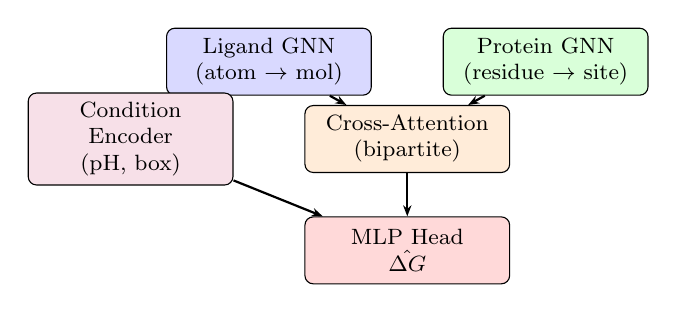
\begin{tikzpicture}[
  box/.style={rectangle, draw=black, rounded corners=3pt,
    minimum width=2.6cm, minimum height=0.85cm, align=center,
    font=\footnotesize},
  arr/.style={-{Stealth[length=4pt]}, thick},
  node distance=0.55cm and 0.9cm
]
  \node[box, fill=blue!15] (lig) {Ligand GNN\\(atom $\to$ mol)};
  \node[box, fill=green!15, right=of lig] (prot) {Protein GNN\\(residue $\to$ site)};
  \node[box, fill=orange!15, below=of $(lig)!0.5!(prot)$] (cross) {Cross-Attention\\(bipartite)};
  \node[box, fill=purple!12, left=of cross] (cond) {Condition\\Encoder\\(pH, box)};
  \node[box, fill=red!15, below=of cross] (mlp) {MLP Head\\$\hat{\Delta G}$};
  \draw[arr] (lig) -- (cross);
  \draw[arr] (prot) -- (cross);
  \draw[arr] (cond) -- (mlp);
  \draw[arr] (cross) -- (mlp);
\end{tikzpicture}
\caption{Schematic of a dual-encoder heterogeneous GNN with cross-attention
(Model~B family).  Ligand and protein sub-graphs are processed by independent
encoders; cross-attention fuses bipartite interaction edges; condition
features (pH, docking box) are concatenated before the regression MLP.
Models~A and~D share a single-encoder GATv2 backbone (Section~\ref{sec:gnn}).}
\label{fig:gnn_arch}
\end{figure}

% ── Fig. 6: Interaction diagram ──────────────────────────────────────────
\begin{figure}[H]
\centering
\includegraphics[width=0.88\textwidth,trim=300 0 90 280,clip]%
  {images/Fig_BS2_interaction_diagram.png}
\caption{Protein--ligand interaction diagram for gallic acid at
GLU\_cluster22 ($\Delta G = -5.10$\,kcal/mol; pH~5.0).
Six simultaneous contacts: ARG496/499 (H-bonds), GLY497/722 (backbone NH),
LYS723 ($\varepsilon$-ammonium), GLU724 (salt bridge).}
\label{fig:interaction}
\end{figure}

% ══════════════════════════════════════════════════════════════════════════════

\section*{Acknowledgment}
% ══════════════════════════════════════════════════════════════════════════════

The authors thank the Fujii Laboratory, Department of Civil and Environmental
Engineering, School of Environment and Society, Institute of Science Tokyo,
for support and research environment.  N.~Darumas acknowledges the Royal Thai
Government Scholarship.

% ══════════════════════════════════════════════════════════════════════════════
%  References
% ══════════════════════════════════════════════════════════════════════════════

\begin{thebibliography}{00}

\bibitem{hermanson2013bioconjugate}
G.~T.~Hermanson, \emph{Bioconjugate Techniques}, 3rd~ed.
London, U.K.: Academic Press, 2013.

\bibitem{carvalho2023gallic}
D.~N.~Carvalho \emph{et al.}, ``Gallic acid as a natural phenolic crosslinker
for collagen-based scaffolds: Physicochemical characterisation and
\emph{in vitro} cytocompatibility,''
\emph{Int. J. Biol. Macromol.}, vol.~236, Art.~no.~123912, 2023,
doi:~10.1016/j.ijbiomac.2023.123912.

\bibitem{haslam1998practical}
E.~Haslam, \emph{Practical Polyphenolics: From Structure to Molecular
Recognition and Physiological Action}.
Cambridge, U.K.: Cambridge Univ. Press, 1998.

\bibitem{jumper2021alphafold}
J.~Jumper \emph{et al.}, ``Highly accurate protein structure prediction with
AlphaFold,'' \emph{Nature}, vol.~596, pp.~583--589, 2021,
doi:~10.1038/s41586-021-03819-2.

\bibitem{koes2013lessons}
D.~R.~Koes, M.~P.~Baumgartner, and C.~J.~Camacho, ``Lessons learned in
empirical scoring with smina from the CSAR 2011 benchmarking exercise,''
\emph{J. Chem. Inf. Model.}, vol.~53, no.~8, pp.~1893--1904, 2013,
doi:~10.1021/ci300604z.

\bibitem{quiroga2016vinardo}
R.~Quiroga and M.~A.~Villarreal, ``Vinardo: A scoring function based on
AutoDock Vina improves scoring, docking and virtual screening,''
\emph{PLOS ONE}, vol.~11, no.~5, Art.~no.~e0155183, 2016,
doi:~10.1371/journal.pone.0155183.

\bibitem{olsson2011propka}
M.~H.~M.~Olsson \emph{et al.}, ``PROPKA3: Protein pK$_{a}$ predictions for
proteins in explicit solvent,'' \emph{J. Chem. Theory Comput.}, vol.~7,
no.~2, pp.~525--537, 2011, doi:~10.1021/ct100578z.

\bibitem{berman2000protein}
H.~M.~Berman \emph{et al.}, ``The Protein Data Bank,''
\emph{Nucleic Acids Res.}, vol.~28, no.~1, pp.~235--242, 2000,
doi:~10.1093/nar/28.1.235.

\bibitem{warren2006critical}
G.~L.~Warren \emph{et al.}, ``A critical assessment of docking programs and
scoring functions,'' \emph{J. Med. Chem.}, vol.~49, no.~20,
pp.~5912--5931, 2006, doi:~10.1021/jm050362n.

\bibitem{orgel2006fibril}
J.~P.~R.~O.~Orgel \emph{et al.}, ``Microfibrillar structure of type~I
collagen \emph{in situ},'' \emph{Proc. Natl. Acad. Sci. USA}, vol.~103,
no.~24, pp.~9001--9005, 2006, doi:~10.1073/pnas.0502718103.

\bibitem{hopkins2014le}
A.~L.~Hopkins, G.~M.~Keser\"u, P.~D.~Leeson, D.~C.~Rees, and
C.~H.~Reynolds, ``The role of ligand efficiency metrics in drug discovery,"
\emph{Nat. Rev. Drug Discov.}, vol.~13, no.~2, pp.~105--121, 2014,
doi:~10.1038/nrd4163.

\bibitem{gilmer2017mpnn}
J.~Gilmer, S.~S.~Schoenholz, P.~F.~Riley, O.~Vinyals, and G.~E.~Dahl,
``Neural message passing for quantum chemistry,'' in \emph{Proc. 34th
Int. Conf. Mach. Learn. (ICML)}, Sydney, Australia, 2017, pp.~1263--1272.

\bibitem{schutt2018schnet}
K.~T.~Sch\"{u}tt, H.~E.~Sauceda, P.-J.~Kindermans, A.~Tkatchenko, and
K.-R.~M\"{u}ller, ``SchNet -- a deep learning architecture for molecules
and materials,'' \emph{J. Chem. Phys.}, vol.~148, no.~24,
Art.~no.~241722, 2018, doi:~10.1063/1.5019779.

\bibitem{kendall2018multi}
A.~Kendall, Y.~Gal, and R.~Cipolla, ``Multi-task learning using
uncertainty to weigh losses for scene geometry and semantics,'' in
\emph{Proc. IEEE Conf. Comput. Vis. Pattern Recognit. (CVPR)},
Salt Lake City, UT, USA, 2018, pp.~7482--7491,
doi:~10.1109/CVPR.2018.00781.

\bibitem{sundararajan2017axiomatic}
M.~Sundararajan, A.~Taly, and Q.~Yan, ``Axiomatic attribution for deep
networks,'' in \emph{Proc. 34th Int. Conf. Mach. Learn. (ICML)},
Sydney, Australia, 2017, pp.~3319--3328.

\bibitem{selvaraju2017grad}
R.~R.~Selvaraju, M.~Cogswell, A.~Das, R.~Vedantam, D.~Parikh, and
D.~Batra, ``Grad-CAM: Visual explanations from deep networks via
gradient-based localization,'' in \emph{Proc. IEEE Int. Conf. Comput.
Vis. (ICCV)}, Venice, Italy, 2017, pp.~618--626,
doi:~10.1109/ICCV.2017.74.

\bibitem{abnar2020quantifying}
S.~Abnar and W.~Zuidema, ``Quantifying attention flow in transformers,''
in \emph{Proc. 58th Annu. Meeting Assoc. Comput. Linguistics (ACL)},
2020, pp.~4190--4197, doi:~10.18653/v1/2020.acl-main.385.

\end{thebibliography}

\end{document}
